\chapter{Produktvorarbeit}
\section{Untersuchungen}
\subsection{Pfaditechniken}

Der Inhalt der App werden die Pfaditechniken sein, welche in sechs Themen aufgeteilt sind: Pionier, Karte und Kompass, Übermittlung, Natur und Umwelt, Samariter und Pfadigeschichte. Die meisten Informationen aus den folgenden Unterkapiteln sind aus den Büchern Thilo\cite{noauthor_thilo_2014} und Technix\cite{muller_technix_2007}.

\subsection*{Pionier}

Bei Pionier geht es rund um Seile, Knoten, Blachen und Zelte. Dabei ist wichtig, dass es nicht nur darum geht, wie man sie benutzt, sondern auch, wie man sie pflegt und was für Vorteile und Nachteile welches Material mit sich bringt.

\subsubsection*{Seile}

Bei den Seilen unterscheidet man zwischen vier Seilarten: Hanfseile, Bergseile, Statikseile und Polypropylenseile. Polypropylenseile sind dabei für Pionierarbeiten zu vernachlässigen, da diese schnell schmelzen. Die anderen Seilarten haben folgende Eigenschaften:
\begin{center}
\begin{table}[!h]
\begin{tabularx}{\textwidth}{p{0.2\textwidth}|X|X|X}
     & \textbf{Hanfseil} & \textbf{Bergseil} & \textbf{Statikseil} \\ \hline
     Merkmal & braun, gedreht & farbig, geflochten & farbig, geflochten \\\hline
     Anwendung & Pioniertechnik, Seilbrücken & Abseilen & Seilbahnen, Strickleiter \\\hline
     Dehnung & gering & gross & gering \\\hline
     Temperatur- beständigkeit & $\approx$ 200$^\circ$C & $\approx$ 100$^\circ$C & $\approx$ 100$^\circ$C \\\hline
     Reissfestigkeit (trocken 10mm) & 800 kg & 2000 kg & 3000 kg \\\hline
     Material & Naturfaser & Kunstfaser (Nylon, Polyamid) & Kunstfaser (Nylon) \\\hline
     Scheuerfestigkeit & gut & empfindlich & gut \\\hline
     Verrotungs- beständigkeit & schlecht & gut & gut \\\hline
     Wasseraufnahme & viel (verkürzt sich) & wenig & wenig \\
\end{tabularx}
\caption{Seilarten und ihre Eigenschaften}
\end{table}
\end{center}
\newpage
Die Seilpflege ist ein weiterer sehr wichtiger Aspekt, wenn es um Seile geht, damit diese lange halten und auch sicher für den Gebrauch sind. \\Die fünf wichtigsten Grundsätze sind:
\begin{enumerate}
\item Stehe nicht auf Seile
\item Reinige Seile regelmässig (trocken)
\item Schütze Seile vor Schmutz, Feuchtigkeit und direkter Sonnenbestrahlung
\item Lagere Seile trocken und vor Sonnenlicht geschützt
\item Lasse Seile nie über scharfe Kanten laufen
\end{enumerate}

\subsubsection{Knoten}

Genau wie bei den Seilen gibt es auch bei den Knoten einige Punkte, auf die man achten sollte:
\begin{itemize}
\item Befestige alle Knoten
\item Ein Knoten halbiert die Tragfähigkeit eines Seiles
\item Lasse am Knotenende genügend freies Seil
\item Bringe einen Stecken beim Knoten zwischen die Verbindung, um den Knoten nach der Belastung wieder öffnen zu können.
\end{itemize}

\begin{center}
\begin{table}
\begin{tabularx}{\textwidth}{X|X|X|X}
\textbf{Name} & \textbf{Verwendung} & \textbf{Positive Eigenschaften} & \textbf{Negative Eigenschaften} \\\hline
Samariter & Verbindung gleich dicker Seile & Einfach, flach, leicht straffzuziehen & Öffnet sich bei grosser Belastung \\\hline
Weber & Verbindung ungleich dicker Seile & Einfach zu knüpfen, leicht straffzuziehen & Öffnet sich bei grosser Belastung \\\hline
Fischer/Spierenstich & Verschiebbare Verbindung zweier ungleich dicker Seile & Hält sicher, kleine Verringerung der Reissfestigkeit & Mühsam zu öffnen \\\hline
Gesteckter Achter & Schlinge zum Anseilen & Hält sicher, gut zum Öffnen & - \\\hline
Bretzeli & Seilbefestigung an dünnen Gegenständen & Schnell geknüpft & Mühsam zu öffnen \\\hline
Maurer & Seilbefestigung an dicken Gegenständen & Einfach zu öffnen & Nur eine Zugrichtung, hält nur bei Belastung \\\hline
Fläschli/Päckli & Zulaufende Schlinge für Pakete, Spanner, Strickleitern & Einfach zu knüpfen & Nur eine Schlaufe und Zugrichtung, mühsam zu öffnen \\\hline
Fuhrmann & Zulaufende Schlinge für Spanner & Besser lösbar als Fläschli/Päckli & Nur eine Schlaufe und Zugrichtung, mühsam zu öffnen \\\hline
Anker & Befestigung einer Schlaufe & Einfach zu knüpfen & Seitliches Verrutschen, gleicher Zug an beiden Enden \\\hline
Halbmastwurf & Abseilen von Lasten & Gute Kontrolle von Lasten & Schnell falsch geknüpft, schwere Handhabung \\\hline
Achterschlinge/ Mastwurf & Fixieren eines Seiles & Hält sehr gut, schräger Zug möglich & Mühsam zu öffnen \\\hline
Schachbrett-/ Freundschaftsknoten & Zierknoten zum Binden der Pfadikrawatte & Flacher Knoten & Mühsam zu öffnen \\
\end{tabularx}
\caption{Tabelle mit den wichtigsten Knoten und ihren Eigenschaften}
\end{table}
\end{center}

\newpage

\subsubsection{Blachen und Zelte}
Bei den Pfadfindern werden häufig Zelte mit Blachen und Zelteinheiten gebaut. Mit Zelteinheiten sind Säcke mit 3 Zeltstangen und 3 Heringen gemeint. Mit Blachen sind Militärblachen gemeint, welche eine Fläche von circa 1.63 m$\times$1.65 m haben. Blachen sind circa 1.25kg schwer (nass bis zu 2.5kg) und haben 32 Löcher und 64 Knöpfe. Bei Blachen ist die Pflege sehr wichtig, schmutzige Blachen soll man zuerst trocknen lassen und danach abbürsten. Ausserdem soll man nicht auf Blachen treten und sie nicht waschen, da beides ihre Imprägnierung kaputt macht. Dies ist eine Tabelle mit den häufigsten Anwendungen von Blachen:

\begin{center}
\begin{table}[h]
\begin{tabularx}{\textwidth}{X|X|X|X}
    \textbf{Name} & \textbf{Anwendung} & \textbf{Material} & \textbf{Hinweise} \\\hline
    Blachenbund & Lagerung von 10 Blachen & 10 Blachen & - \\\hline
    Sarg & Gepäckunterstand, Windschutz für 1 Person & 1 Blache, 2 Zelteinheiten, Schnur & Sehr klein \\\hline
    Gotthardschlauch & Schlafstelle für 3 Personen, Materialunterstand & 3 Blachen, 2 Zelteinheiten, Schnur & Ist beliebig erweiterbar \\\hline
    Firstzelt & Gepäckunterstand & 2 Blachen, 2 Zelteinheiten, Schnur & Ist beliebig erweiterbar \\\hline
    Berliner & Schlafstelle für 5 Personen & 8 Blachen, 4 Zelteinheiten, Schnur & Wärmstes Blachenzelt \\\hline
    Sarasani & Aufenthaltszelt, Kochzelt & 27 Blachen, 1 Mittelpfosten, Schnur, 2 Seile, 15 Armierungseisen & Kann beliebig vergrössert werden \\ 
\end{tabularx}
\caption{Die häufigsten Anwendungen von Blachen}
\end{table}
\end{center}

\subsection*{Karte und Kompass}
\subsubsection{Grundsatz}
Die Schweiz hat ein eigenes Koordinatensystem, welches nach der Sternwarte Bern (2 600 000 \\/1 200 000) ausgerichtet ist. Das Schweizer Koordinatensystem ist zudem rechteckig was bedeutet, dass jeder Punkt der Schweiz mit einer x und einer y Koordinate angegeben werden kann. Bei den Karten der Schweiz ist Norden immer oben und sie sind in acht Massstäbe unterteilt,\newline 1:10 000, 1:25 000, 1:50 000, 1:100 000, 1:200 000, 1:300 000, 1:500 000 und 1:1 000 000. Der Massstab ist hierbei $\frac{Kartenstrecke}{Naturstrecke}$. Für die Pfadfinder sind allerdings praktisch nur die 1:25 000 und 1:50 000 relevant, da sie nicht so weite Strecken zurücklegen. Auf Karten werden ausserdem Höhenkurven verwendet, welche es dem Benutzer ermöglichen anhand einer Karte abzuschätzen wie steil ein Gelände ist. Zwischen zwei Höhenkurven liegt eine konstante Äquidistanz, welche zwischen 10m und 50m variiert. 

\subsubsection{Koordinaten bestimmen}
Zum Bestimmen der Koordinaten eines Punktes auf der Karte verwendet man einen Kartenmassstab. Als ersten Schritt sucht man die Grobkoordinaten des Feldes in welchem der Punkt sich befindet den man sucht. Danach liest man mit dem Kartenmassstab die genauen Koordinaten der x und y Achse ab. \par Um einen Punkt mithilfe von Koordinaten zu finden sucht man zuerst das Feld in dem der Punkt liegt und bestimmt anschliessend den Ort des Punktes in dem man die genauen x und y Werte mithilfe des Kartenmassstabs in die Karte einträgt.

\subsubsection{Signaturen}

Signaturen auf einer Karte sind Symbole, welche für ein Objekt in der realen Welt stehen. So entspricht zum Beispiel ein einfaches Quadrat auf einer Karte einem Haus. Diese Signaturen helfen, dass man sich in einer unbekannten Umgebung mit einer Karte zurechtfinden kann. Auf der Kartenrückseite gibt es ein Verzeichnis der wichtigsten Signaturen. Die Signaturen können zusätzlich auch online gefunden werden\cite{oa_zeichenerklarung_nodate}.

\subsection*{Samariter/Erste Hilfe}
Beim Samariter geht es darum in der Not erste Hilfe leisten zu können. Das korrekte Vorgehen ist wichtig. Als verständnishilf gibt es ein Ampelsystem. Rot bedeutet schauen. Das Ausmass des Unfalls abschätzen und sich selbst vor Gefahren zu schützen. Orange bedeutet denken. Einen Handlungsplan erstellen. Grün bedeutet handeln. Es wird umgesetzt was bei Orange geplant wurde. \par
Beim Handeln ist das Alarmieren ein wichtiger Punkt. Alarmieren kann über Tod und Leben entscheiden. Pfadfinder lernen die wichtigsten Notrufnummern: 112 für den Europäischen Notruf, 117 für die Polizei, 118 für die Feuerwehr, 144 für die Ambulanz, 1414 für die REGA und 145 für das Tox-Zentrum. Dazu die wichtigsten Fragen der Alarmierung: Wer?, Was?, Wo?, Wann?, Wieviele? und Weiteres?. \par
Nach dem Alarmieren kümmert man sich um den Patient, hierbei gibt es die Regel ABC. A steht für Atemwege, hier wird geschaut, ob der Patient in der Lage ist zu Atmen. B steht für Beatmen, dies wird durchgeführt, wenn der Patient nicht mehr atmet. C steht für CPR was eine Herzmassage ist, diese wird durchgeführt, wenn das Beatmen keine Wirkung zeigt. \par
Falls die Atmung funktioniert und ein Patient starke Blutungen oder Schmerzen hat, muss man teilweise einen Verband machen. Es gibt drei Arten: Einen Druckverband, einen Stützverband oder einen Deckverband. Der Druckverband übt starken Druck auf die Wunde aus und kann so starke Blutungen stoppen. Der Stützverband dient als Stütze für ein verletztes Körperteil. Der Deckverband dient als Schutz vor Verunreinigungen der Wunden.

\subsection*{Übermittlung}
Die Übermittlung befasst sich hauptsächlich mit dem Morsecode, hier werden Buchstaben in Punkt und Strich codiert und so versendet. Der grosse Vorteil von Morsen ist, dass man verschiedene Arten anwenden kann, zum Beispiel mit Morsetafeln oder mit Taschenlampen im Dunkeln. Zur Codierung von Buchstaben zu Morsecode wird ein Morseschlüssel verwendet \cref{fig:Morseschlüssel}.
\begin{figure}[h]
    \centering
    \includegraphics[width=\linewidth]{Picture/morseschlüssel.png}
\caption{Morseschlüssel \\ \url{https://de.scoutwiki.org/Morsen}}
\label{fig:Morseschlüssel}
\end{figure}
\par
Ein weiterer Aspekt der Übermittlung sind die Geheimschriften. Im Thilo \cite{noauthor_thilo_2014} sind mehrere dieser Verschlüsselungsarten: Die Cäsarverschlüsselung, bei der alle Buchstaben um eine bestimmte Anzahl Buchstaben im Alphabet verschoben werden. Das Quadratgitter, hierbei schreibt man die Nachricht waagrecht in ein Raster und sendet sie danach Senkrecht gelesen. Das Koordinatengitter, hierbei wird das Alphabet in ein Koordinatengitter geschrieben, danach bekommt jede Zeile und Spalte einen Buchstaben als Koordinate. Die Nachricht ist danach die Koordinaten aller Buchstaben der Nachricht zusammen gehängt.
\subsection*{Pfadigeschichte}
Robert Stephenson Smyth Baden-Powell, der Gründer der Pfadfinderbewegung, wurde am 22. Februar 1857 in London geboren. Er fiel durch die Aufnahmeprüfungen der Universität und entschied sich Karriere im Militär zu machen. Er wurde in der Kolonie Indien stationiert wo er auf Spione oder Scouts aufmerksam wurde und deren wichtige Funktion im Kampfgeschehen erkannte. Später wurde er nach Südafrika verlegt, wo er zum ersten Mal seine eigenen Scouts ausbildete, aber immer noch im militärischen Umfeld. Als Baden-Powell, nun besser bekannt als BiPi, eine Stadt aus der Belagerung befreien musste, setzte er seine Scouts erstmals im Gefecht ein und er war erstaunt, wie gut sie ihre Aufgaben bewältigten. \par Zurück in England beendete BiPi seine Militärische Karriere und sagte: \glqq Am Ende meiner Karriere begann ich, die Kunst, junge Leute zu lehren, wie man Krieg macht, umzuwandeln in die Kunst junge Leute zu lehren, in Frieden zu leben; Pfadi ist weit entfernt vom Krieg\grqq\cite{noauthor_thilo_2014}(Zitiert nach: Thilo S. 24) \par
Im Jahre 1907 organisierte er das erste Pfadilager für Jungen auf der Insel Brownsea. Nach dem riesigen Erfolg dieses Lagers schrieb er das Buch Pfadfinder. Das Buch war ein solcher Erfolg, dass überall in England neue Pfadigruppen entstanden und 1909 auch Mädchenabteilungen entstanden unter dem Namen Guides. \par Im Jahre 1912 heiratete BiPi Olave Saint Clair Soames, welche als Chief Guide die Leitung der Pfadfinderinnen übernahm. 1920 fand das erste Jamboree\footnote{Pfadilager mit Abteilungen von der ganzen Welt} statt, es nahmen Jugendliche aus 34 Ländern teil. Später wurde BiPi zum World Chief ernannt. Die Pfadibewegung explodierte und um 1993 gab es etwa 25 Millionen Pfadi in über 150 Ländern.

\subsection*{Natur und Umwelt}

Bei Natur und Umwelt geht es darum zu wissen wie man richtig Recycelt und dass man die wichtigsten einheimischen Tiere und Tierspuren kennt.

\subsubsection{Recycling}

\textbf{PET-Flaschen: }Aus PET-Flaschen können neue PET-Flaschen hergestellt werden, daher ist es sehr wichtig diese zu recyceln. PET-Flaschen gehören in die blau-gelb markierten Mülltonen. Plastikflaschen wie Milch-, Öl-, Essig-, Saucen- und Shampooflaschen, Getränkekartons (z. B. Tetra Pak) und andere Verpackungen aus PET gehören nicht in die PET-Sammlung. Vor dem Entsorgen, sollte aus der Flasche immer die Luft raus gelassen werden, damit die einzelne Flasche weniger Platz benötigt. \par

\textbf{Plastikflaschen: }Plastikflaschen können im Gegensatz zu PET-Flaschen nicht wieder zu Flaschen werden, aber aus ihnen entstehen andere Produkte. Plastikflaschen können in Lebensmittelläden wie Coop oder Migros abgegeben werden. PET-Getränkeflaschen, halbvolle Plastikflaschen, Getränkekartons (z. B. Tetra Pak), Plastikflaschen aus dem Heimwerker-, Garten- und Autobereich, Schalen, Becher, Tuben, Folien, Nachfüllbeutel gehören nicht zu den Plastikflaschen. Vor dem Entsorgen, sollte aus der Flasche immer die Luft raus gelassen werden, damit die einzelne Flasche weniger Platz benötigt. \par

\textbf{Batterien: }Batterien bestehen aus seltenen Rohstoffen, welche zurückgewonnen werden können, wenn man sie recycelt. Sie sind rückgabenpflichtig und gehören nicht in den Abfall. Batterien können in den meisten Läden an der Kasse oder in der Recyclingstation des Ladens abgegeben werden. \par

\textbf{Elektrische und elektronische Geräte: }Elektrische und elektronische Geräte enthalten wertvolle Ressourcen welche wiederverwendet werden können. Elektrische und elektronische Geräte können auf den meisten Recyclinghöfen der Gemeinden entsorgt werden oder dank der vorgezogenen Recyclinggebühr an den Verkaufsstellen zurückgegeben werden. \par

\textbf{Glas: }Glas kann unendlich viele Male Recycelt werden. Zur idealen Verwertung muss das Glas nach Farben getrennt werden. Glas sollte vor dem Recyceln ausgespült werden und danach nach Farben sortiert bei einem Glascontainer entsorgt werden. Getrennt werden: Weiss-, Grün- oder Braunglas. Alle anderen Farben gehören zum Grünglas. \par

\textbf{Aluminium: }Aluminium kann unendlich viele Male Recycelt werden, deshalb ist es sehr wichtig, dass man es recycelt. Aluminium kann direkt bei Aluminium-Sammelstelle der Gemeinde abgegeben werden. Das Aluminium sollte gepresst werden um Platz zu sparen. \par

\textbf{Karton: }Aus Karton kann wieder Karton hergestellt werden und so kann Holz gespart werden. Karton kann meist direkt bei der Karton-Sammelstelle der Gemeinde abgegeben werden. \par

\textbf{Papier: }Aus Papier kann Zeitungspapier oder auch Karton gemacht werden. Papier kann bei der Altpapier-Sammelstelle der Gemeinde abgegeben werden. \par

\textbf{Kleidung: }Kleidung ist oft in so gutem Zustand, dass sie nochmal getragen werden kann und in Secondhandläden weiterverkauft wird. Aus nicht mehr tragbarer Kleidung werden Putzlumpen und Füllmaterial gemacht. Alle Kleidungstücke können in Kleidersäcken gesammelt werden und bei Kleidercontainer oder Strassensammlungen abgegeben werden \cite{noauthor_migros_2024}.

\subsubsection{Einheimische Tiere}

Bei den einheimischen Tieren geht es überwiegend darum die wichtigsten Tiere zu erkennen. Ausserdem wird zu jedem Tier noch ein kurzer Steckbrief geschrieben. \par

\textbf{Igel: }Rücken mit vielen Stacheln. Körper eher Plump. Grösse: 22-28. In der Dämmerung und Nachts aktiv. Frisst Würmer, Insekten, Schnecken, Obst. Echter Winterschläfer. Lebt in Gebüschen, an Waldrändern, in Gärten. \par

\textbf{Maulwurf: }Schwarzes, samtiges Fell. Walzenförmiger Körper. Sehr kleine, mit Fell versteckte Augen. Vorderfüsse wie Grabschaufeln. Grösse: 11-15 cm. Lebt unterirdisch. Wirft lose Erde zu Haufen auf. Frisst Würmer, Insekten, kleine Wirbeltiere. Lebt in Gärten, Feldern und Wäldern. \par

\textbf{Spitzmaus: }Schnauze lang und spitz wie ein Rüssel. Samtiges, braunes bis graues Fell. Grösse: 5-10 cm. Frisst Würmer, Kerbtiere. Lebt fast überall, in Häusern, Feld und Wasser.\par

\textbf{Fledermaus: }Mit grosser, dünner Flughaut, die zwischen je 4 verlängerten Fingern, Armen, Beinen und Schwanz ausgespannt ist. Daumen kurz, mit Kralle. Fell dunkelbraun bis grau. Grösse: 3-8 cm. In der Dämmerung und Nacht aktiv. Ruht am Tag aufgehängt an den Hinterbeinen auf Dachböden, in hohlen Bäumen und Höhlen. Winterschläfer. \par

\textbf{Feldhase: }Gelbbraunes Fell. Ohrenspitzen und Schwanzoberseite sind schwarz. Er legt in Bodenvertiefungen Lager an. Ohren mindestens so lang wie Kopf und lange kräftige Beine, er macht oft Männchen zur Fluchtsicherung. Grösse: 48-68 cm. Frisst Pflanzen. Lebt in Feldern, Wiesen, an Waldrändern.\par

\textbf{Eichhörnchen: }Langer, buschiger Schwanz und vor allem im Winter Haarbüschelchen an den Ohren. Zehen mit langen gebogenen Krallen (gewandter Kletterer und Springer). Rotbraunes oder schwarzes Fell. Tagtier. Hält keinen Winterschlaf. Frisst Nüsse, Zapfen, Knospen und auch Vogeleier. Lebt in Wäldern, Parkanlagen und Gärten.\par

\textbf{Feldmaus: }Bräunliches Fell, glatter Schwanz, kleine Ohren, stumpfe Schnauze. Als Wühlmaus gräbt sie unterirdische Gänge und Höhlen. Grösse: 9-12 cm. Vorwiegend Pflanzenfresser. Lebt in Feldern, Gärten, Wiesen.\par

\textbf{Gemse: }Hörner am Ende hakig gebogen. Dunkelbraunes Fell, Kopf und Hintern weiss. Klettert und springt sehr gut. Ihre Sprünge erreichen oft 7 bis 9 m Länge. Tagtier. Nahrung: Gras, Blätter, junge Triebe an Ästen. Lebensraum: Hochgebirge bis 3000 m Höhe, steile Weisen und felsige Gebiete.\par

\textbf{Steinbock: }Graubraunes Fell. Mächtiges schön geschwungenes Gehörn, mit dicken Querwülsten auf der Vorderseite beim Männchen. Die Geiss hat kürzere Hörner. Tagaktiv in kleinen Rudeln. Klettert und springt sehr gut. Pfeifender Warnruf. Frisst Pflanzen. Lebt in den Alpen oberhalb der Baumgrenze.\par

\textbf{Reh: }Rötlichbraunes Sommerkleid, graubraunes Winterkleid. Im Sommer lebt das Reh allein oder in kleinen Gruppen, im Winter dagegen in Rudeln von 10-20 Tieren. Der Rehbock trägt ein kleines Geweih, das er im Winter abwirft. Das Reh hat im Gegensatz zum Hirsch keinen Schwanz. Frisst frische Blätter, Gras und Eicheln. Lebt in Wäldern, auf Feldern mit viel Gebüsch und auf Wiesen.\par

\textbf{Rothirsch: }Rotbraunes Sommerkleid, braungraues Winterkleid. Er hat einen kleinen Schwanz, den er auf der Flucht hoch hält, wobei das weisse Hinterteil sichtbar wird. Das kräftige Stangengeweih wird jedes Jahr abgeworfen. Lautes Röhren als Brunftschrei. Dämmerungs- und nachtaktiv. Pflanzenfresser. Lebt in grösseren Wäldern und im Gebirge bis über die Waldgrenze.\par

\textbf{Fuchs: }Rotbraunes Fell. Kopf- und Brustunterseite und Schwanzspitze sind weiss. Dämmerungs- und nachtaktiv. Lebt einzeln oder familienweise in selbstgebauten Höhlen (Fuchsbau). Frisst Mäuse, Beeren, Insekten und Geflügel. Lebt in Wald, Feld und Gebüsch. \par

\textbf{Dachs: }Bräunlichgraues Fell, Kopf schwarzweiss längsgestreift. Er gräbt sich eine Höhle mit weitläufigen, komplizierten Gängen. Dämmerungs- und nachtaktiv. Lebt paarweise. Im Winter ist seine Tätigkeit ziemlich verlangsamt, er macht aber keinen eigentlichen Winterschlaf. Allesfresser. Lebensraum: Wälder und Gebüsch.\par

\textbf{Steinmarder: }Braunes Fell. am Hals weiss. Dämmerungs- und nachtaktiv. Klettert und springt sehr gut. Frisst Vögel, Mäuse, Insekten, Beeren. Lebt in Wäldern, Siedlungs- und Feldgebieten.\par

\textbf{Stockente: }Männchen: Grüner Kopf, graubraune Federn, weisser Halsring und gelber Schnabel. Weibchen: Graubrauner Körper, Orangener Schnabel. Lebt fast überall wo es Gewässer hat. Frisst überwiegend pflanzliche Stoffe.\par

\textbf{Kuckuck: }Graue Federn. Bekannt für den Kuckucksruf. Legt seine Eier in fremde Nester. Wohnt überwiegend im Wald und in Kulturlandschaften. Frisst Insekten.\par

\textbf{Grünspecht: }Oberseite grün, unterseite hell- bis graugrün gefärbt, Kopf ist teilweise rot. Wohnt an Waldrändern und Parks mit Bäumen. Frisst Ameisen mit seiner 10 cm langen Zunge.\par

\textbf{Grünfink: }Gelbe Federn, beim Schwanz grau-schwarz. Lebt in kleinen Dörfern und in Städten. Frisst Schoten, Kapseln und Früchte.\par

\textbf{Uhu: }Hell- bis dunkelbraune Federn, orange Augen, Federohren. Lebt vor allem im Mittelgebirge und den Alpen. Frisst kleine bis mittelgrosse Säugetiere und Vögel.\par

\textbf{Rotmilan: }Brauner Körper, Flügel schwarz und weiss, gegabelter Schwanz. Lebt im Sommer in Mitteleuropa und im Winter in Südwesteuropa. Frisst kleine Säugetiere, wirbellose Tiere, Amphibien, kleine Vögel und Aas. \par

\textbf{Mäusebussard: }Dunkelbraunes bis fast Weisses Gefieder, abgerundeter Schwanz. Lebt auf Wiesen und Äckern mit angrenzendem Wald. Frisst überwiegend kleine Säugetiere.\par

\textbf{Turmfalke: }Rotbraune Flügeloberseite, Weisser Körper und Flügelunterseite, Männchen: Grauer Kopf, Weibchen: Rotbrauner Kopf. Lebt in Waldrändern, auf Hochspannungsleiungen oder in Gebäuden. Frisst Mäuse und Singvögel.\par

\textbf{Ringelnatter: }Häufig in der Nähe von Wasser. Färbung grau, mit zwei leuchtendgelben, halbmondförmigen Fleken hinter dem Kopf. Bis 1.5m lang. Kann schwimmen. Lebt von Fröschen und Fischen.\par

\textbf{Kreuzotter: }Schwarze Zickzackzeichnung auf rotbraunem Grund, kantiger Kopf und flache Schnauzenspitze. Ist giftig. Bis 80 cm lang. Lebt vorwiegend in feuchten Wiesen, Waldrändern und Kahlschlägen. \par

\textbf{Feuersalamander: }Runder Schwanz. Keine Schwimmhäute zwischen den Zehen. Glänzend schwarz, mit gelben Flecken oder Streifen. \par

\textbf{Erdkröte: }Der Körper ist braun oder grau. Nur zur Laichzeit im Wasser zu finden, sonst in Gärten, Feldern und Wäldern. Tagsüber in Erdhöhlen, nachts aktiv. \par

\textbf{Grasfrosch: }Stumpfe Schnauze. Nur an den Hinterbeinen Schwimmhäute. Die Oberseite ist braun mit dunklen Flecken und einem grossen dunklen Schläfenfleck.


\subsection{Java}
Die Programmiersprache dieses Projektes ist Java. Java existiert seit 1995. In dieser Sprache werden viele Apps programmiert\cite{oa_what_nodate}. Java ist so aufgebaut, dass wenn ein Programm darin läuft, eine virtuelle Maschine gestartet wird. Dies hat zur Folge, dass bei einem Fehler nicht der Computer, der das Programm ausführt abstürzt, sondern die virtuelle Maschine\cite{wikipedia-autoren_java_2024}. Java ist eine Programmiersprache, welche für die \gls{oop} entwickelt wurde. 

\subsubsection{Wichtige Syntax}
In Java gibt es wichtige Grundbegriffe die man beherrschen sollte, um die Funktion der Java-Programme zu verstehen. Entscheidend ist, zum Beispiel dass am Ende einer Zeile mit einer Anweisung ein Semikolon gesetzt wird und dass der Code innerhalb von Funktionen immer in geschweiften Klammern geschrieben ist. Ein weiterer wichtiger Punkt ist, dass man eine Klasse und eine Main Methode hat in der man das Programm schreibt. Um in einem Programm etwas auszugeben schreibt man System.out.println(\dq Text\dq);\cite{programmieren_lernen_java_2021}.
\begin{minted}{java}
//Die Main Klasse ist die Hauptklasse des Programms
public class Main {
    //Die Main Methode ist der Einstiegspunkt in das Programm
    public static void main(String[] args) {
        System.out.println("Hello World!");
        //Diese Programm liefert den Output: Hello World!
    }
}
\end{minted}

\subsubsection{Datentypen}
Die Datentypen in Java sind in 2 Kategorien aufgeteilt: Primitive Datentypen und Referenzen Datentypen. Primitive Datentypen gibt es acht Byte, Short, Integer, Long, Float, Double, Character und Boolean. Die ersten vier Datentypen sind dabei für die ganzzahligen Zahlen verantwortlich, hierbei kann in einem Byte eine Zahl im Bereich von $-2^7$ bis $2^7-1$ gespeichert werden, in einem Short eine Zahl im Bereich von $-2^{15}$ bis $2^{15}-1$, in einem Integer eine Zahl im Bereich von $-2^{31}$ bis $2^{31}-1$ und in einem Long eine Zahl im Bereich von $-2^{63}$ bis $2^{63}-1$. Somit ist es nur eine Frage des Speicherplatzes und der Grösse der Zahl, welchen dieser Datentypen man nimmt. Als Standard wird meist der Integer als Mittelwert verwendet. In diesen Datentypen können aber keine Kommazahlen gespeichert werden, diese werden in einem Float oder in einem Double gespeichert. Diese beiden Datentypen unterscheiden sich im Bereich an Zahlen, die sie speichern können. Ein Float deckt den Bereich von $\pm 1.4 \cdot 10^{-45} \text{bis} \pm 3.4 \cdot 10^{38}$ ab und ein Double den Bereich von $\pm 4.9 \cdot 10^{-324} \text{bis} \pm 1.7 \cdot 10^{308}$. Hier hat sich als Standard der Double durchgesetzt.\par 
Die zwei verbleibenden Datentypen sind der Character und der Boolean. Der Character kann Zeichen in sich Speichern, es ist allerdings nicht nur möglich Buchstaben des lateinischen Alphabets zu verwenden, es gehen auch Zahlen, Spezialzeichen wie @ oder Unicode wie $\backslash$03A9 für $\Omega$. Der letzte primitive Datentyp ist der Boolean. Ein Boolean hat nur zwei Status True und False oder in Computersprache 1 und 0 \cite{studyflix_java_nodate}.\par
Der zweite Typ von Datentypen sind die Referenzen Datentypen, zu ihnen gehören alle anderen Datentypen wie zum Beispiel Klassen und ihre Objekte, Interfaces, Arrays, Strings, etc. All diese Datentypen setzen sich aus mehreren Primitiven Datentypen zusammen, so sind Strings zum Beispiel einfach viele Character aneinander gehängt.

\subsubsection{Variablen}
In Java gibt es wie in den meisten Programmiersprachen Variablen. Der Nutzen von Variablen ist das Speicher von Werten. Der Wert einer Variable kann überschrieben werden, der Datentyp des Wertes muss aber gleich bleiben. Variablen müssen immer deklariert und definiert werden, damit man sie benutzen kann. Dies kann in zwei unterschiedlichen Zeilen geschehen oder in einer.
\begin{minted}{java}
public class Main {
    public static void main(String[] args) {
        int integerValue;
        //Deklarierung der Variable intergerValue
        //Zuerst wir der Datentyp definiert, dann der Variablenname
        integerValue = 1;
        //Definition der Variable intergerValue
        //Der Variablenname ist gleich dem gewünschten Variablenwert
        double doubleValue = 1.0;
        //Deklaration und Definition der Variable doubleValue in einem Schritt
        //Zuerst wird der Datentyp genannt, dann der Variablenname ist gleich 
        //dem gewünschten Variablenwert
    }
}
\end{minted}
Variablen können ausserdem miteinander zusammengerechnet oder zusammengeführt werden\cite{programmieren_lernen_java_2021}.
\begin{minted}{java}
public class Main {
    public static void main(String[] args) {
        int intValue = 1;
        //Hier wird eine Variable mit dem Namen intValue und dem Wert 1 erstellt
        int intValue2 = 2;
        //Hier wird eine Variable mit dem Namen intValue2 und dem Wert 2 erstellt
        int intValue3 = intValue + intValue2;
        //Hier wird eine Variable mit dem Namen intValue3 und dem Wert von 
        //intValue + intValue2 erstellt
    }
}
\end{minted}

\subsubsection{Verzweigungen}
Verzweigungen in Programmiersprachen sind dafür da verschiedene Szenarien zu unterscheiden und für jedes Szenario den richtigen Programmabschnitt auszuführen. Hier gibt es zwei Hauptmethoden, die verwendet werden: If, Else Anweisung und Switch case. Die If Else Anweisung vergleicht zwei Werte. Ergibt der Vergleich, dass sie identisch sind wird der If Teil der Funktion durchgeführt sind sie nicht identisch, wird der Else Teil durchgeführt. In einem optionalen dritten Teil dem Else-If Teil, wird ein weiterer Vergleich durchgeführt um eine andere Übereinstimmung zu finden.
\begin{minted}{java}
public class Main{
    public static void main(String[] args) {
        if (2 == 1){
            //Wenn 2 gleich 1 ist, dann wird das ausgeführt
        } else if (2 == 2) {
            //Wenn 2 gleich 2 ist, dann wird das ausgeführt
        } else {
            //Wenn nichts davon zutrifft, dann wird das ausgeführt
        }
    }
}
\end{minted}
Die andere häufig verwendete Methode des Switch cases macht im Grundsatz genau das Gleiche. Hier wird eine Variable in den Switch Teil hinein gegeben, die dann für verschiedene Werte Überprüft wird. Anschliessend wird der zum Wert passende Programmabschnitt ausgeführt\cite{programmieren_lernen_java_2021}.
\begin{minted}{java}
public class Main{
    public static void main(String[] args) {
        int var;
        switch (var) {
            case 1:
                //Wenn die Variable var den Wert 1 hat, wird dieser Code 
                //ausgeführt
                break;
            case 2:
                //Wenn die Variable var den Wert 2 hat, wird dieser Code 
                //ausgeführt
                break;
            default:
                //Wenn die Variable var keinen der Werte 1 oder 2 hat, 
                //wird dieser Code ausgeführt
        }
    }
}
\end{minted}

\subsubsection{Schleifen}
Schleifen in der Programmierung lassen gewisse Zeilen eines Programms mehrfach ausführen. Genau wie bei den Verzweigungen gibt es hier zwei Typen von Schleifen, die sich durchgesetzt haben: die While und die For Schleife. Die While Schleife macht einen Teil des Programms so lange, bis eine Bedingung nicht mehr erfüllt ist. Die For schleife wiederholt einen Teil des Programms so lange, bis sie durch alle Glieder einer bestimmten Reihe oder eines Arrays durch ist oder bis die Variable, die man der Schleife gibt einen bestimmten Wert übersteigt\cite{freecodecamporg_android_2020}(Zeit: 1:47:43). \clearpage
\begin{minted}{java}
public class Main{
    public static void main(String[] args) {
        
        int count = 0;
        while (count < 10) {
            //Solange die Bedingung count ist kleiner als 10 erfüllt ist, wird
            //der Code wiederholt
            //Hier ist der Code der wiederholt werden soll
            count++;
            //Count wird um 1 erhöht und es wird wieder geprüft, ob die 
            //Bedingung erfüllt ist
        }
        
        for (int i = 0; i < 10; i++) {
            //Solange die Bedingung i kleiner als 10 erfüllt ist, wird der 
            //Code wiederholt, i wird um 1 erhöht
            //Hier ist der Code der wiederholt werden soll
        }
        String word = "Hallo";
        for (char c : word.toCharArray()) {
            //Solange es noch Zeichen im Wort gibt, wird der Code wiederholt
            //Hier ist der Code der wiederholt werden soll
        }
    }
}
\end{minted}

\subsubsection{Klassen und Objekte}
Java ist eine Sprache, die auf die \gls{oop} ausgelegt wurde. Die \gls{oop} definiert eine Klasse und mit den Objekten dieser Klasse kann weiter programmiert werden. Innerhalb einer Klasse gibt es sogenannte Methoden. Methoden sind Teile eines Programms, die ein Objekt dieser Klasse ausführen können. So könnte man zum Beispiel eine Figuren Klasse erstellen, mit der Methode jump, welche auslöst dass die Figur springt. Die Klasse erlaubt uns, dass wir mehrere Figuren haben, die alle über die Methode jump verfügen. Den Methoden der Klasse können dann auch noch Atribute mitgegeben werden welche dann den Output beeinflussen können. So kann zum Beispiel der Methode Jump noch eine Sprunghöhe mitgegeben werden
\clearpage
\begin{minted}{java}
//Datei: Main.java
public class Main{
    public static void main(String[] args) {
        //Ein neues Objekt der Klasse Figuren wird erstellt mit dem Namen Mario
        Figuren Mario = new Figuren("Mario");
        //Die Methode jump() wird aufgerufen über das Objekt Mario, der Methode
        //wird die Zahl 3 mitgegeben welche dann in dem Attribut hoehe 
        //gespeichert wird
        Mario.jump(3);

        //Ein neues Objekt der Klasse Figuren wird erstellt mit dem Namen Luigi
        Figuren Luigi = new Figuren("Luigi");
        //Die Methode jump() wird aufgerufen über das Objekt Luigi, der Methode
        //wird die Zahl 1 mitgegeben welche dann in dem Attribut hoehe 
        //gespeichert wird
        Luigi.jump(1);
    }
}

//Datei: Figuren.java
public class Figuren {
    private String name;

    public Figuren(String name){
        this.name = name;
    }

    public void jump(int hoehe){
        System.out.println(name + " springt" + hoehe + " m hoch");
    }
}

//Output:
//Mario springt 3 m hoch
//Luigi springt 1 m hoch
\end{minted}

\subsection{Android Studio}
Android Studio ist eine Desktop App für die Entwicklung von Android Apps. In Android Studio kann entweder in Java oder in Kotlin programmiert werden. Android Studio ist eine JetBrains IDE \footnote{Integrated development environment} was bedeutet, dass es man eine direkte Verbindung mit GitHub aufbauen kann, um so das Projekt auf GitHub stets auf dem neusten Stand zu haben.

\subsubsection{Struktur}
Innerhalb von Android Studio gibt es drei Arten von Dateien, welche miteinander verbunden sind. Die Ressource Dateien, die Layout Dateien und die Java Dateien. Die Ressource Dateien sind Dateien wie Bilddateien oder Themendateien welche die Grundlage der Informationen bilden auf der die ganze App basiert. Die Layout Dateien erstellen Objekte auf dem Bildschirm des Users. So steht zum Beispiel in einer Layout Datei, wo ein Button ist, was er für einen Hintergrund hat, wie er heisst und wie gross er ist. In den Java Dateien werden den Objekten aus den Layout Dateien Funktionen gegeben. Hier wird das Programm geschrieben, das ausgeführt wird, wenn man einen Button drückt\cite{freecodecamporg_android_2020}(Zeit: 7:26:53).

\subsubsection{Layouts}
Bei den Layouts in Android Studio gibt es Unterschiede. So gibt es drei Hauptarten von Layouts: Das Constraint Layout, das Relative Layout und das Linear Layout. Bei dem Constraint Layout werden die Objekte immer mit Verbindungen zu anderen Objekten positioniert. Beim Relative Layout werden die Objekte immer relativ zu den anderen positioniert, so wird hier häufig mit Abständen zu anderen Objekten gearbeitet. Beim Linear Layout werden die Objekte immer in einer fixen Reihe positioniert und es kann nur der Abstand zum vorherigen Objekt verändert werden. Bei all diesen Layouts müssen die Attribute der Objekte identisch in den Layoutdateinen angegeben werden\cite{freecodecamporg_android_2020}(Zeit: 6:58:39).
\newpage
\section{Entwurf}
Als Entwurf der App wurde ein Prototyp erstellt. Dieser zeigt wie die App im finalen Stadium aussehen könnte und wie ihre grobe Struktur sein wird.
\begin{figure}[h]
    \centering
    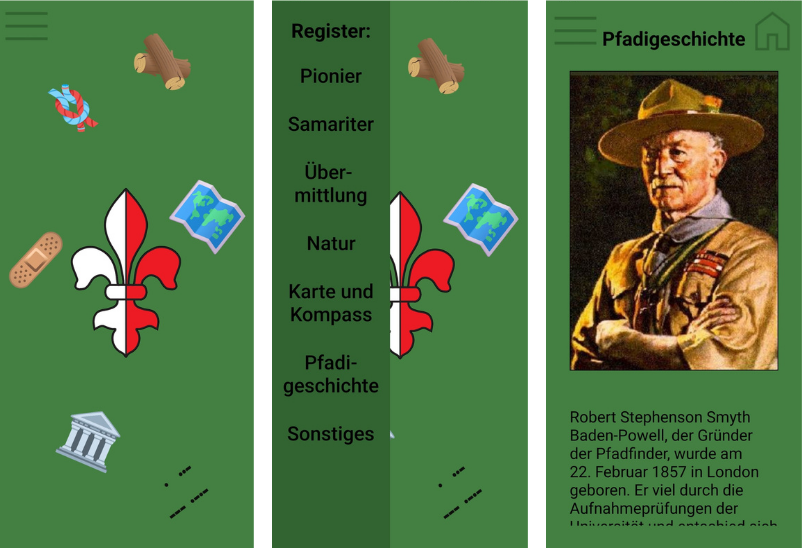
\includegraphics[width=\linewidth]{Picture/homescreen.png}
    \caption{Bildschirmaufnahmen des Prototyps}
\end{figure}
Hier sieht man, wie der Homescreen (links) der App aufgebaut ist. In der Mitte steht die Pfadililie und rund herum sind einige Image Buttons mit den jeweiligen Themen angeordnet. Alle Themen sind hier mit einem für sie symbolischen Bild vertreten ausser der Bereich Sonstiges. Diese Bilder fungieren als Buttons welche den User zu den Informationsseiten des jeweiligen Themas bringt. Ein weiteres Element auf dem Homescreen ist der Hamburger Button in der oberen linken Ecke. Er öffnet das Register (mitte). Beim Register sind alle Themen aufgelistet und man kann durch das Anklicken dieser Wörter zu den jeweiligen Seiten kommen.\par
Die Informationsseiten (rechts) werden wie folgt aufgebaut sein. Oben links wird weiterhin der Hamburger Button sein, um das Register zu öffnen. Auf der rechten Seite wird neu ein Homebutton sein welcher zurück zum Homescreen führt. Zwischen diesen Buttons wird der Titel stehen, hier als Beispiel Pfadigeschichte. Darunter kommt in den meisten Fällen ein Bild oder eine Graphik, bevor die eigentlichen Informationen beginnen.
\newpage
\begin{center}
\begin{figure}[h]
    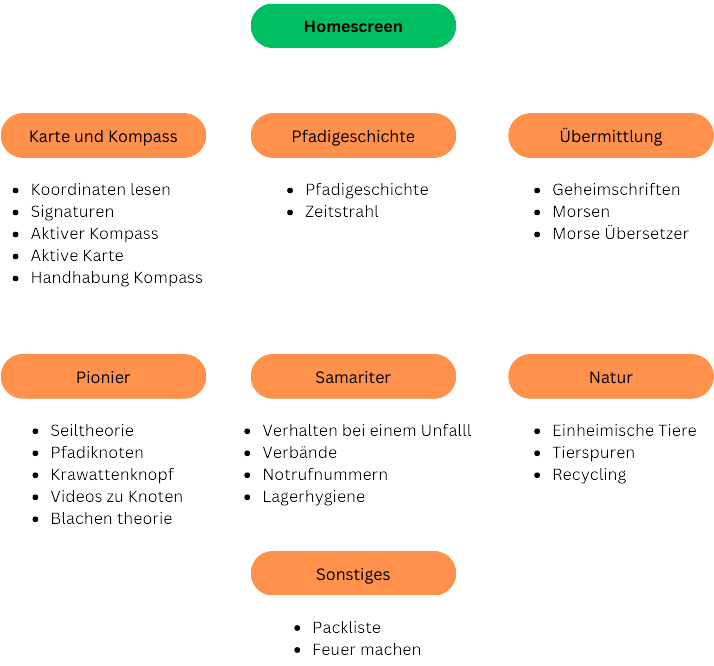
\includegraphics[width=1\linewidth]{Picture/appstruktur.png}
    \caption{Aufbau der App}
\end{figure}
\end{center}
Die App wird so Strukturiert sein, dass man zuerst auf dem Homescreen (grün) landet, danach kann man über das Register oder die Image Buttons in die einzelnen Themen (orange). In diesen Themen, kann man dann schlussendlich in die Unterthemen in denen die einzelnen detaillierten Informationen sind.